\chapter{Geometria del Profilo}

La geometria di un Profilo Sesta Serie NACA Laminare è data in forma tabellare a partire dal profilo simmetrico e dalla linea media standard.\\ I punti di partenza per la disegnazione tecnica del profilo NACA $66_4-221$ sono stati tratti dal  H. ABBOTT (1958) \cite{prof:abbott}.\\ 

\begin{figure}[H]
\centering
\begin {minipage} [c] {.40\textwidth}
\centering\setlength{\captionmargin}{0pt}%
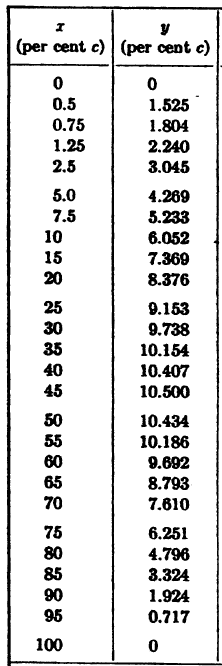
\includegraphics[width=.63\textwidth]{immagini/simmetrico.png}      % 
\caption{Profilo $66_4-021$} %
\end{minipage}
\hspace{13mm}%
\begin {minipage} [c] {.40\textwidth}
\centering\setlength{\captionmargin}{0pt}%
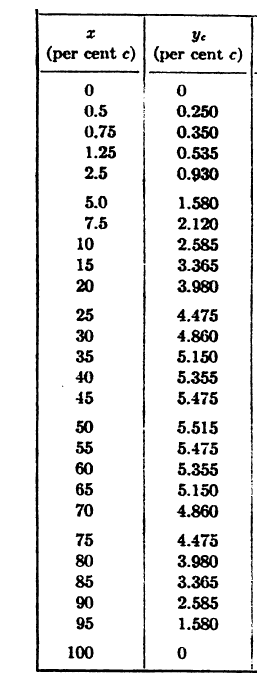
\includegraphics[width=.63\textwidth]{immagini/lineamedia.png}      % 
\caption{Linea media standard} %
\end{minipage}
\end{figure}

\newpage 

\begin{figure} [H]
\centering
\begin{tikzpicture} 
\begin{axis} [ 
xmin=0, 
xmax=1, 
ymin=-0.15,
 ymax=0.15,
 xlabel=$ \frac {x}{c}$, 
ylabel=$ \frac {z}{c}$,
ytick={-0.15,-0.1,-0.05,0,0.05,0.1,0.15},
yticklabels={$-0.15$,$-0.1$,$-0.05$,$0$,$0.05$,$0.1$,$0.15$},
width=13cm,
 height=3.9 cm,
scale only axis,
grid=major] 
\addplot [black,very thick,smooth]
file{immagini/punti_664221_pane.dat};
\addplot [black,very thick,smooth]
file{immagini/lineamedia_NACA664221.dat};
\end{axis}
\end{tikzpicture}
\caption{\footnotesize Profilo  NACA $66_4-221$ }
\end{figure}

\noindent \\

Il disegno tecnico del profilo NACA $66_4-221$ è stato eseguito a partire dai punti del profilo simmetrico NACA $66_4-021$ e di quelli della linea media standard, questi ultimi opportunamente scalati per tener conto del $C_{li}=0.2$. Di seguito sono riportati i disegni necessari per quanto concerne la costruzione del profilo stesso.\\

\begin{figure} [H]
\centering
\begin{tikzpicture} 
\begin{axis} [ 
xmin=0, 
xmax=1, 
ymin=-0.15,
 ymax=0.15,
 xlabel=$ \frac {x}{c}$, 
ylabel=$ \frac {z}{c}$,
ytick={-0.15,-0.1,-0.05,0,0.05,0.1,0.15},
yticklabels={$-0.15$,$-0.1$,$-0.05$,$0$,$0.05$,$0.1$,$0.15$},
width=13cm,
 height=3.9 cm,
scale only axis,
grid=major] 
\addplot [black, mark=*,only marks]
file{immagini/profilo_simmetrico_NACA664021.dat};
\end{axis}
\end{tikzpicture}
\caption{\footnotesize Profilo simmetrico per punti NACA $66_4-021$ }
\end{figure}

\begin{figure} [H]
\centering
\begin{tikzpicture} 
\begin{axis} [ 
xmin=0, 
xmax=1, 
ymin=-0.1,
 ymax=0.1,
 xlabel=$ \frac {x}{c}$, 
ylabel=$ \frac {z}{c}$,
ytick={-0.1,-0.05,0,0.05,0.1},
yticklabels={$-0.1$,$-0.05$,$0$,$0.05$,$0.1$},
width=13cm,
 height=2.6 cm,
scale only axis,
grid=major] 
\addplot [black, mark=*]
file{immagini/lineamedia_NACA664221.dat};
\end{axis}
\end{tikzpicture}
\caption{\footnotesize linea media a=1 $C_{li}=0.2$ }
\end{figure}

\begin{figure} [H]
\centering
\begin{tikzpicture} 
\begin{axis} [ 
xmin=0, 
xmax=1, 
ymin=-0.15,
 ymax=0.15,
 xlabel=$ \frac {x}{c}$, 
ylabel=$ \frac {z}{c}$,
ytick={-0.15,-0.1,-0.05,0,0.05,0.1,0.15},
yticklabels={$-0.15$,$-0.1$,$-0.05$,$0$,$0.05$,$0.1$,$0.15$},
width=13cm,
 height=3.9 cm,
scale only axis,
grid=major] 
\addplot [black, mark=*,only marks]
file{immagini/punti_profilo_664221.dat};
\end{axis}
\end{tikzpicture}
\caption{\footnotesize Profilo per punti NACA $66_4-221$ }
\end{figure}

\begin{figure} [H]
\centering
\begin{tikzpicture} 
\begin{axis} [ 
xmin=0, 
xmax=1, 
ymin=-0.15,
 ymax=0.15,
 xlabel=$ \frac {x}{c}$, 
ylabel=$ \frac {z}{c}$,
ytick={-0.15,-0.1,-0.05,0,0.05,0.1,0.15},
yticklabels={$-0.15$,$-0.1$,$-0.05$,$0$,$0.05$,$0.1$,$0.15$},
width=13cm,
 height=3.9 cm,
scale only axis,
grid=major] 
\addplot [black, mark=*,only marks]
file{immagini/punti_profilo_664221.dat};
\addplot [black,very thick,smooth]
file{immagini/punti_664221_pane.dat};
\addplot [black,very thick,smooth]
file{immagini/lineamedia_NACA664221.dat};
\end{axis}
\end{tikzpicture}
\caption{\footnotesize Confronto punti con interpolante profilo NACA $66_4-221$ }
\end{figure}

\begin{figure} [h!]
\centering
\begin{tikzpicture} 
\begin{axis} [ 
xmin=0.9, 
xmax=1.02, 
ymin=-0.03,
 ymax=0.03,
 xlabel=$ \frac {x}{c}$, 
ylabel=$ \frac {z}{c}$,
%xtick={-0.03,0,0.03,0.06,0.09},
width=13cm,
 height=6.5 cm,
scale only axis,
grid=major] 
\addplot [black,very thick,smooth]
file{immagini/punti_664221_pane.dat};
\end{axis}
\end{tikzpicture}
\caption{\footnotesize Profilo alare NACA $66_4-221$. Zoom del bordo d'uscita }
\end{figure}

\begin{figure} [h!]
\centering
\begin{tikzpicture} 
\begin{axis} [ 
xmin=-0.02, 
xmax=0.05, 
ymin=-0.05,
 ymax=0.05,
 xlabel=$ \frac {x}{c}$, 
ylabel=$ \frac {z}{c}$,
xtick={-0.03,0,0.03,0.06,0.09},
width=6.3cm,
height=9 cm,
scale only axis,
grid=major] 
\addplot [black,very thick,smooth]
file{immagini/punti_664221_pane.dat};
\end{axis}
\end{tikzpicture}
\caption{\footnotesize Profilo alare NACA$66_4-221$. Zoom del bordo d'attacco }
\end{figure}

Tramite xfoil è stata ricavato l'andamento della curvatura del profilo in funzione dell'ascissa curvilinea, riportato nelle figure che seguono.\\

\begin{figure} [H]
\centering
\begin{tikzpicture} 
\begin{axis} [ 
xmin=0, 
xmax=2.02, 
ymin=-2.6,
 ymax=60,
 xlabel=$ \frac {s}{c}$, 
ylabel=$ curvatura$,
width=11cm,
 height=7 cm,
scale only axis,
grid=major] 
\addplot [black,solid,very thick]
file{immagini/curvatura_laminare.dat};
\end{axis}
\end{tikzpicture}
\caption{\footnotesize NACA $66_4221$- Andamento ascissa curvilinea - curvatura }
\end{figure}
\noindent
 \\ \\

\begin{figure} [H]
\centering
\begin{tikzpicture} 
\begin{axis} [ 
xmin=0, 
xmax=2.02, 
ymin=-2.6,
 ymax=2.5,
 xlabel=$ \frac {s}{c}$, 
ylabel=$ curvatura$,
width=11cm,
 height=7 cm,
scale only axis,
grid=major] 
\addplot [black,solid,very thick]
file{immagini/curvatura_laminare.dat};
\end{axis}
\end{tikzpicture}
\caption{\footnotesize  NACA $66_4-221$ -Andamento ascissa curvilinea - curvatura, zoom }
\end{figure}
\noindent
 \\

 Al fine di migliorare la geometria, i punti di ascissa ({\bfseries X}), ordinata({\bfseries Y}) e ascissa curvilinea del profilo ({\bfseries S}),  sono stati importati in MATLAB ed elaborati con un codice in grado di generare delle {\itshape spline} X(S) e Y(S) ed interpolarle al fine di ottenere 100 punti sul dorso e 100 punti sul ventre, alle stesse ascisse.

\begin{figure} [h!]
\centering
\begin{tikzpicture} 
\begin{axis} [ 
xmin=0, 
xmax=2.02, 
ymin=0,
 ymax=1,
 xlabel=$ \frac {s}{c}$, 
ylabel=$ \frac {x}{c}$,
width=12cm,
 height=5.5 cm,
scale only axis,
grid=major] 
\addplot [black,solid,very thick]
file{immagini/acissa_ascissacurvilinea_laminare.dat};
\end{axis}
\end{tikzpicture}
\caption{\footnotesize NACA $66_4-221$ Andamento ascissa curvilinea - ascissa }
\end{figure}


\begin{figure} [h!]
\centering
\begin{tikzpicture} 
\begin{axis} [ 
xmin=0, 
xmax=2.02, 
ymin=-0.1,
 ymax=0.15,
 xlabel=$ \frac {s}{c}$, 
ylabel=$ \frac {z}{c}$,
width=12cm,
 height=6 cm,
scale only axis,
ytick={-0.1,-0.05,0,0.05,0.1,0.15},
yticklabels={$-0.1$,$-0.05$,$0$,$0.05$,$0.1$,$0.15$},
grid=major] 
\addplot [black,solid,very thick]
file{immagini/ordinata_ascissacurvilinea_laminare.dat};
\end{axis}
\end{tikzpicture}
\caption{\footnotesize NACA $66_4-221$ Andamento ascissa curvilinea - ordinata}
\end{figure}
\noindent  \\ 

I punti del profilo sono stati importati sul software CAD CATIA V5 per rappresentare l’ala infinita, con profilo costante, di elevato allungamento.\\

\begin{figure} [h!]
\centering
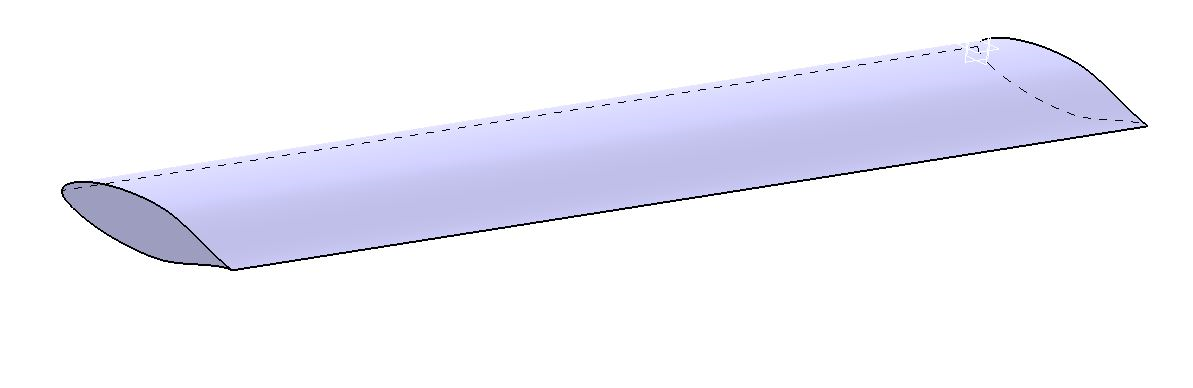
\includegraphics  [ height=5cm] {immagini/fig11.png}
\caption{\footnotesize Ala infinita, profilo costante NACA $66_4-221$, rendering in CATIA V5}
\end{figure}

